% !TeX root = ../Rules.tex
% !TeX spellcheck = en_US
\section{Laws of the Game}

\law{1}{The Field of Play}
\label{sec:field}

% ADDED BY REINALDO

The competition consists of three distinct divisions, categorized specifically by the maximum physical height and weight of the robotic platforms.

To ensure a fair and proportionate competitive environment, the field dimensions, number of players and ball size will vary to align with the specific requirements of each division (see \Cref{sec:divisions} for more details).

\sublaw{Field surface}
\label{sec:field_surface}

The matches are played on artificial turf with a height between approximately 20 to 30 mm, except for the small division, which has a height between 8 and 12 mm, also approximately.

The color of artificial turf must be green. No particular shade is required, but the green must contrast well with the field markings and the ball and should not be very dark.

\sublaw{Field markings}
\label{sec:field_markings}

The field of play must be rectangular and marked with continuous lines.
These lines belong to the areas of which they are boundaries.

The color of the field markings should be white, whether applied by tape, paint, or made from white turf.

The two longer boundary lines are called touchlines (or sidelines). The two shorter lines are called goal lines.
The field of play is divided into two halves by a halfway line, which joins the midpoints of the two touchlines.

A team's half is the half of the field that is closest to the team's own goal, where it primarily defends against opposing attacks.

The center mark is at the midpoint of the halfway line. A circle is marked around it, defining the center circle, a region used for kick-offs and other specific plays.

The goal area and the penalty area are defined using lines drawn at right angles to the goal line.

All lines must be of the same width, which must be between 5 and 12 cm.

\Cref{fig:field_line_names} shows the field markings with the lines and its names.

\begin{figure}[h]
    \centering
    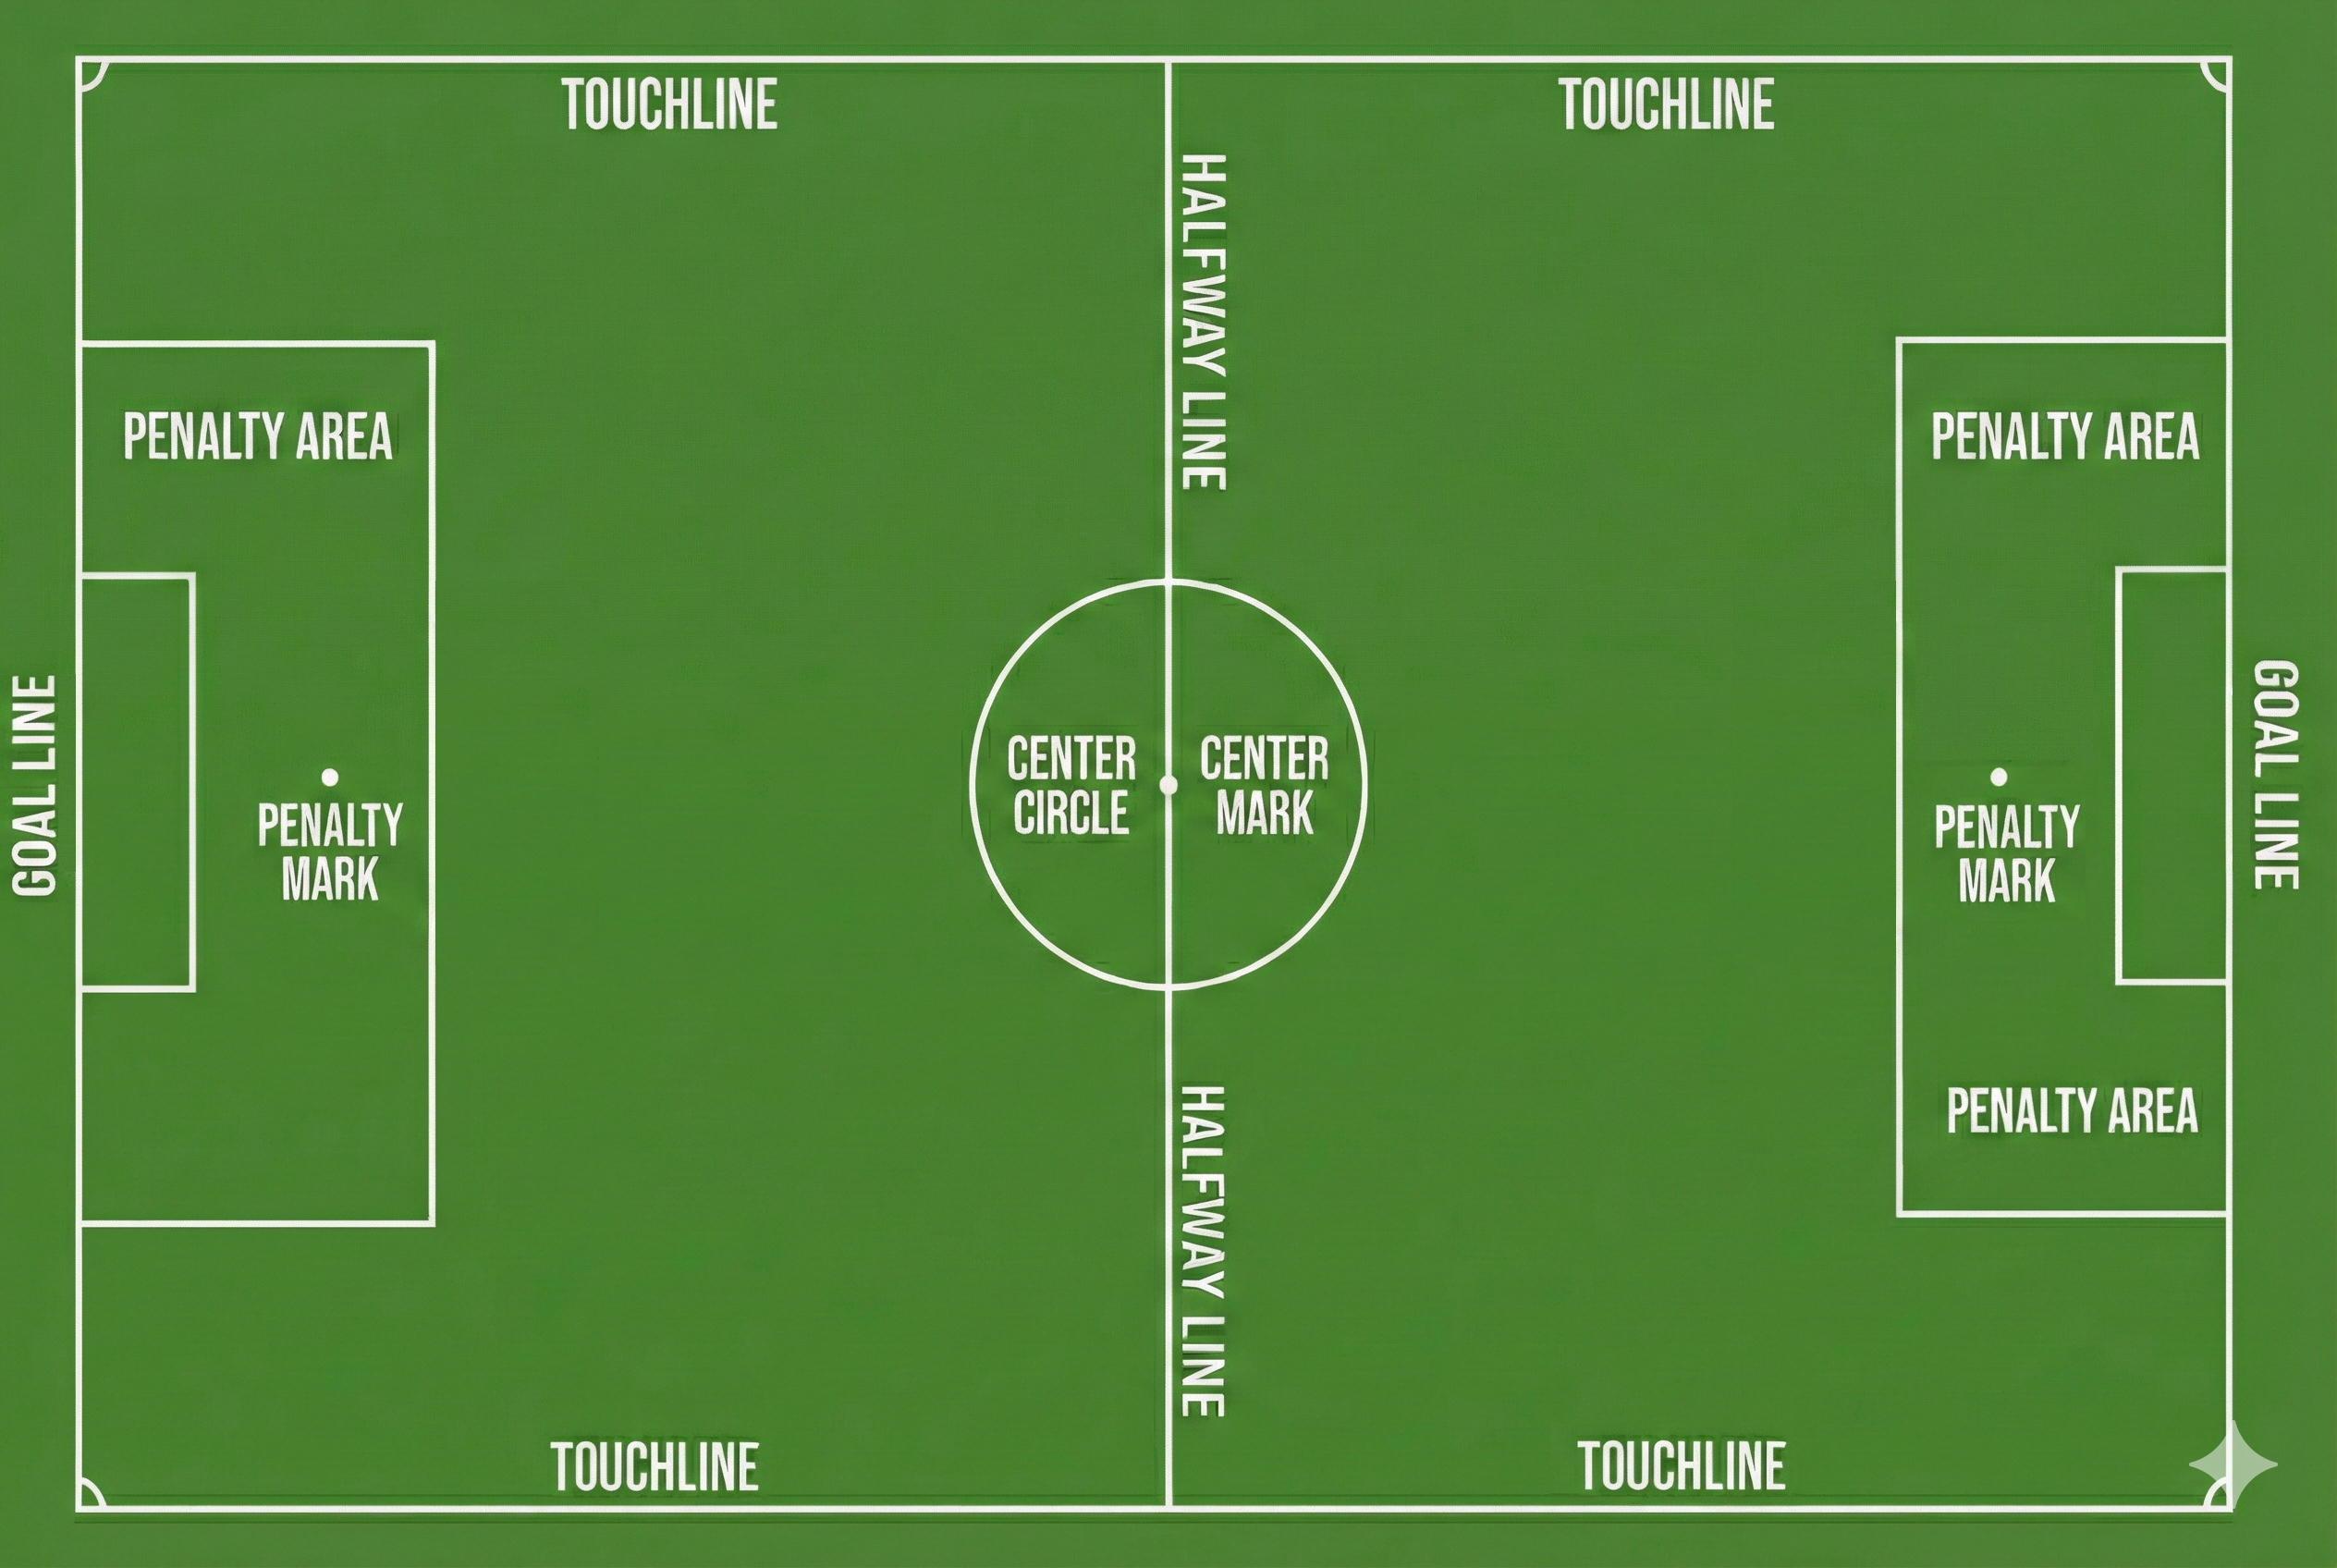
\includegraphics[width=0.7\columnwidth]{figs/Figure-1-line-names.png}
    \caption{Annotated diagram illustrating the standard markings and key areas of a soccer field.}      
    \label{fig:field_line_names}
\end{figure}

\sublaw{The goal area}
\label{sec:goal_area}

Two lines are drawn at right angles to the goal line; the length and distance from the midpoint of the goal line depend on the division.

These lines extend into the field of play and are joined by a line drawn parallel with the goal line.
The area bounded by these lines and the goal line is the goal area.

\sublaw{The penalty area}
\label{sec:penalty_area}

Two lines are drawn at right angles to the goal line; the length and distance from the midpoint of the goal line depend on the division.

These lines extend into the field of play and are joined by a line drawn parallel with the goal line.
The area bounded by these lines and the goal line is the penalty area. 

Within each penalty area, a penalty mark is made. 

\sublaw{The corner arc}
\label{sec:corner_arc}

A quarter circle from each corner is drawn inside the field of play.
The radius of the arc is 0.5m for the M-Field and 1.0m for the L-Field. The S-Field does not have corner arcs.

\sublaw{Dimensions}
\label{sec:dimensions}

There are three field sizes that can be used for the proposed divisions, described in \Cref{tab:field_dim_rule}.

\begin{table}[h]
    \centering
    \begin{tblr}{
        colspec = {X[l] X[c] X[c]},
        width=\linewidth,
        hlines,
        vlines,
        row{1} = {font=\bfseries}, % header
    }% begin tblr
        Field                  & Width (meters) & Length (meters) \\
        S-Field (small field)  & 6       & 9 \\
        M-Field (middle field) & 6 to 9  & 9 to 14 \\
        L-Field (large field)  & 9 to 14 & 14 to 22 \\
    \end{tblr}
    \caption{Approximate field sizes.}
    \label{tab:field_dim_rule}
\end{table}

\Cref{tab:field_dim} shows the dimensions of the S-, M- and L-Fields.
Diagrams of the three soccer fields are shown in \Cref{fig:field_small,fig:field_medium,fig:field_large}. 
Note that the Middle Division can be played on the S-Field or the M-Field, while the Large Division can be played on both the M-Field and the L-Field.
More detailed technical drawings are provided in \Cref{sec:technical_drawings}.

Note that measurements are from the outside of the lines as the lines are part of the area they enclose (as it is in the FIFA Rules).

\begin{table}[h]
    \centering
    \begin{tblr}{
        colspec = {c l X[c] X[c] X[c]},
        width=\linewidth,
        hlines,
        vlines,
        rows={f}, % align text in the middle 
        row{1} = {font=\bfseries}, % header
        row{2} = {font=\itshape}, % comments
        column{1} = {font=\bfseries}, % ids
    }% begin tblr
        ID & Description & S-Field  & M-Field  & L-Field \\
           & (all values in meters) & (former KidSize and SPL) & (former AdultSize) & (similar to MSL)\\

        A & Field length                 & 9.0 & 14.0 & 22.0 \\ 
        B & Field width                  & 6.0 & 9.0 & 14.0 \\ 
        C & Goal length (depth)          & 0.5 to 1.0 & 0.7 to 1.2 & 1.0 to 2.0 \\
        D & Goal width                   & 1.8 to 1.9 & 2.4 to 2.6 & 2.6 to 3.1 \\
        E & Goal Area length             & 1.0 & 1.0 & 1.0  \\ 
        F & Goal Area width              & 3.0 & 4.0 & 5.0  \\
        G & Penalty Area length          & 2.0 & 3.0 & 3.5  \\ 
        H & Penalty Area width           & 4.0 & 6.0 & 7.0  \\
        I & Penalty Mark distance        & 1.5 & 2.0 & 2.5  \\
        J & Center Circle diameter       & 1.5 & 3.0 & 4.0 \\
        K & Border strip width (min.)    & \SetCell[c=3]{c} 1.0 & & \\ 
        L & Corner Arc radius            & none & 0.5 & 1.0 \\ 
          & Line width                   & \SetCell[c=2]{c} 0.05 & & 0.12 \\
          & Penalty and center mark size & \SetCell[c=2]{c} 0.10 & & 0.15 \\
    \end{tblr}
    \caption{Exemplary field dimensions by field type, in meters.}   
    \label{tab:field_dim}
\end{table}


\begin{figure}[h]
  \centering
  \input{rules/small_field}
  \caption{Schematic diagram of the small soccer field -- S-Field (scale: 1/80)}
  \label{fig:field_small}
\end{figure}

\begin{figure}[h]
  \centering
  \input{rules/medium_field}
  \caption{Schematic diagram of the medium soccer field -- M-Field (scale: 1/100)}
  \label{fig:field_medium}
\end{figure}

\begin{figure}[h]
  \centering
 \input{rules/large_field}
  \caption{Schematic diagram of the large soccer field -- L-Field (scale: 1/150)}
  \label{fig:field_large}
\end{figure}

\sublaw{Goals}
\label{sec:goals}
A goal must be placed on the center of each goal line. 
A goal consists of two vertical posts equidistant from the corners and joined at the top by a horizontal crossbar. 

The goalposts and crossbar must be made of wood, metal, or other approved material and must not be dangerous to the players.

The goalposts and crossbar of both goals must be of the same shape, which must be square, rectangular, round, elliptical, or a hybrid of these options.\info{need a figure how goalposts must be placed on the goal line}

The goalposts and crossbar must have the same width, which is not less than 7 cm and does not exceed 12 cm.
The goalposts and the crossbar must be white. Goal nets and any net supports may be white, gray, or black.

Goals must be anchored securely to the ground. 

Off-the-shelf goals may be used if they satisfy these requirements. 


    

\begin{table}[h]
    \centering
    \begin{tblr}{
        colspec = {X[l] X[c] X[c] X[c]},
        width=\linewidth,
        hlines,
        vlines,
        row{1} = {font=\bfseries}, % header
    }% begin tblr
        Division & Width (meters) & Height (meters) & Depth (meters)\\
        Small    & 1.8 to 1.9 & 1.2 to 1.3 & 0.5 to 1.0 \\
        Middle   & 2.4 to 2.6 & 1.5 to 1.9 & 0.7 to 1.2\\
        Large    & 2.6 to 3.1 & 1.8 to 2.0 & 1.0 to 2.0\\
    \end{tblr}
    \caption{Allowed ranges for goal dimensions.}
    \label{tab:goal_dim}
\end{table}

\sublaw{Definition of Inside and Outside}

\label{sec:inside_outside}
An object (such as a {\color{red} robot} or the ball) \unsure{TW: are there other objects? if not why mentioned this?} is considered \textit{inside} a region of the field if any part of it overlaps or touches the boundary lines that define that region, or if it is fully contained within the region, in the air or on the ground. It is considered \textit{outside} the region only when no part of it, or its downwards projection, remains within or on the boundary lines of that region. This definition applies to any designated area of the field, except the goal (see \Cref{fig:field_line_names}).

\textbf{Exception for the goal:} The ball is only considered \textit{inside} the goal (and thus a goal is scored) if, and only if, the entire ball has wholly crossed the goal-side edge of the goal line \emph{between the goal posts and below the crossbar}, \ie{} when no part of the ball remains on or above the goal line, and the entire ball is within the volume enclosed by the goal frame and the net.
\improvement{TW: This needs to be discussed for robots.}

\improvement{TW: This definition, \textit{for robots} is inconsistent with former-SPL rules. I am unsure about former-HL. Robots are defined as inside/outside an area based on the feet touching (or body touching). The projection of the body has implications for illegal positioning, etc. This also has implications if a robot is "in the air". We haven't seen jumping robots yet.}

\improvement{TW: The terms inside/outside appear to be repeatedly redefined in various places. All should refer back to this section.}

\textbf{Exception for the Goal:} The ball is only considered \textit{inside} the goal (and thus a goal is scored) when the entire ball has wholly crossed the goal-side edge of the goal line, \ie{}, when no part of the ball remains on or above the goal line and the ball is outside the field of play.

\sublaw{Venue Setup}
\label{sec:venue_setup}

Fields may be located close to one another.
Barriers will not necessarily be constructed between adjacent fields to block the robots from seeing other fields, goals, or balls. 
However, barriers will be constructed to block sight between any fields that are not located at least three meters apart.
Hence, for each side of a field that is adjacent to another field, either barriers will separate the fields or at least \qty{3}{\metre} will be between the carpet of adjacent fields.

\sublaw{Lighting Conditions}
\label{sec:lightingConditions}

The \leaguenameabbr does not mandate specific or controlled lighting conditions for a match venue. It is expected that the venue provides reasonable lighting suitable for general visibility (\eg indoor with artificial lighting, outdoor with natural lighting, or a combination of both). 

The lighting conditions depend on the actual venue. Fields should be placed near or under windows where possible. 

Whether window lighting is used or not, ceiling lights should be provided as necessary so that most of the field is at least \qty{300}{\lux} (preferably \qty{400}{\lux}). This lighting may include variations such as glare, brightness, shadows, or mixed lighting conditions that can change throughout the match. 

However, the lighting must be predominantly white, and colored lighting that significantly changes the perceived color of the field or ball is not allowed. 

Teams participating in the \leaguenameabbr are encouraged to design their robots to handle a variety of typical lighting environments that may be encountered during a match. Natural and non-natural light must be free to reach the field. The technical committee can delimit a zone near the field where humans must not stand and where any items blocking the light sources are forbidden.

\law{2}{The Ball}
\label{sec:ball}

\sublaw{Qualities and measurements}
\label{sec:ball-measurements}

All balls must be spherical, made of or resembles the weight, form, movement characteristics and appearance of leather or other suitable material.

The balls for each division\footnote{The TC and OC will decide on only one type of the ball per division that will be used by all teams during the 2026 competition.} are defined in \Cref{tab:balls}.

    

\begin{table}[h]
    \centering
    \begin{tblr}{
        colspec = {X[l] X[l]},
        width=\linewidth,
        hlines,
        vlines,
        row{1} = {font=\bfseries}, % header
    }% begin tblr
        Division & Ball Type\\
        Small    & FIFA Mini Ball\\
        Middle   & FIFA size 3 or 4\\
        Large    & FIFA size 5 \\
    \end{tblr}
    \caption{Balls used in each division}
    \label{tab:balls}
\end{table}


\sublaw{Replacement of a defective ball}

If the ball bursts or becomes defective during the course of a match: the match is stopped. It is is restarted by dropping the replacement ball at the place where the original ball became defective.

If the ball bursts or becomes defective whilst not in play at a kick-off, goal kick, corner kick, free kick, penalty kick or throw-in: the match is restarted accordingly.

If the ball becomes defective during a penalty kick or penalties (penalty shoot-out) as it moves forward and before it touches a player, crossbar or goalposts, the penalty kick is retaken.

The ball may not be changed during the match without the referee’s permission.

\sublaw{Additional balls}
Additional balls which meet the requirements of \Cref{sec:ball-measurements} may be placed around the field of play and their use is under the referee's control.